\titre{Fork :} Dans un systeme UNIX, les nouveaux processus sont toujours créés avec la commande fork(). 
\begin{itemize}
	\item Crée une nouvelle entrée dans la table des processus
	\item Copie de l'espace d'adressage
	\item Copie des descripteurs de fichiers
	\item Retourne
	\begin{itemize}
		\item 0 pour le fils
		\item un nombre positif strict pour le père
	\end{itemize}
\end{itemize}

\titre{Wait :} Le père devrait toujours attendre la fin de l'exécution de son fils avec la fonction waitpid, ou encore wait s'il n'a qu'un seul fils. \\

\titre{Thread :} Par défaut, un processus contient un unique thread (processus = ressource + un thread) \\ 
Créer un nouveau thread, c'est créer une nouvelle pile d'exécution à l'intérieur du même processus. \\ 

\titre{Création d'un thread :} On spécifie une fonction dont l'entête est \code{void* fct(void*)}\\

\titre{Figures correspondantes à la correction du td :}\\

\includegraphics[width=100px]{fig3.pdf}
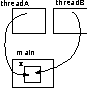
\includegraphics[width=100px]{fig4.pdf} \\\\
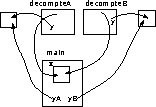
\includegraphics[width=200px]{fig5.pdf} \\\\
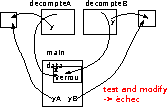
\includegraphics[width=200px]{fig6.pdf}

